\documentclass{article}
\usepackage{amsmath, amssymb}
\usepackage{enumitem}
\usepackage{tikz}
\usetikzlibrary{arrows.meta, positioning}

\setlist[enumerate]{itemsep=1.5em}

\usepackage{titlesec}
\titlespacing*{\section}
{0pt}{1.5ex plus 1ex minus .2ex}{1.3ex plus .2ex}

\usepackage{sectsty}
\sectionfont{\fontsize{12}{15}\selectfont}

\usepackage{geometry}
\geometry{margin=1in}

\begin{document}

\section*{Homework 1 by Amarnath Patel}

\begin{enumerate}

    \item (10 points) Write in words how to read each of the following out loud:
    \begin{enumerate}
        \item $\{x \in \mathbb{R}^+ \mid -1 < x < 1\}$
        
        \vspace{1em}
        The set of all positive real numbers \( x \) such that \( -1 < x < 1 \).
        \vspace{1em}
        
        \hrulefill
        
        \item $\{x \in \mathbb{R} \mid x \leq -3 \text{ or } x \geq 1\}$

        \vspace{1em}
        The set of all real numbers \( x \) such that \( x \leq -3 \) or \( x \geq 1 \).
        \vspace{1em}
        
        \hrulefill

        \item $\{n \in \mathbb{Z} \mid n \text{ is a factor of 3}\}$

        \vspace{1em}
        The set of all integers \( n \) such that \( n \) is a factor of 3.
        \vspace{1em}
        
        \hrulefill

        \item $\{n \in \mathbb{Z}^+ \mid n \text{ is a factor of 5}\}$

        \vspace{1em}
        The set of all positive integers \( n \) such that \( n \) is a factor of 5.
        \vspace{1em}
    \end{enumerate}
    
    \hrulefill

    \item (10 points)
    \begin{enumerate}
        \item Is $3 \in \{3\}$?\\
        \vspace{1em}
        Yes.
        \vspace{1em}
        
        \hrulefill

        \item How many elements are in the set $\{2, 2, 2, 5\}$?\\
        \vspace{1em}
        Two elements.
        \vspace{1em}
        
        \hrulefill

        \item How many elements are in the set $\{0, 0, \{0\}\}$?\\
        \vspace{1em}
        Two elements.
        \vspace{1em}
        
        \hrulefill

        \item Is $\{0\} \in \{\{0\}, 0, \{1\}\}$?\\
        \vspace{1em}
        Yes.
        \vspace{1em}
        
        \hrulefill

        \item Is $0 \in \{\{0\}, \{1\}\}$?\\
        \vspace{1em}
        No.
        \vspace{1em}
    \end{enumerate}
    
    \hrulefill

    \item (10 points) Which of the following sets are equal?
    \begin{align*}
        A &= \{0, 1, 2, 3\} \\
        B &= \{x \in \mathbb{R} \mid -1 \leq x < 4\} \\
        C &= \{x \in \mathbb{R} \mid -1 < x < 4\} \\
        D &= \{x \in \mathbb{Z} \mid -1 < x < 4\} \\
        E &= \{x \in \mathbb{Z}^+ \mid -1 < x < 4\}
    \end{align*}
    \vspace{1em}
    $A = D$ and $D = E$
    \vspace{1em}
    
    \hrulefill

    \item (10 points) Use the set-roster notation to indicate the elements in each of the following sets.
    \begin{enumerate}
        \item $S = \{n \in \mathbb{Z} \mid n = (-1)^k, \text{ for some integer } k\}$\\
        \vspace{1em}
        $S = \{-1, 1\}$
        \vspace{1em}
        
        \hrulefill

        \item $T = \{m \in \mathbb{Z} \mid m = 2 + (-1)^i, \text{ for some integer } i\}$\\
        \vspace{1em}
        $T = \{1, 3\}$
        \vspace{1em}
        
        \hrulefill

        \item $U = \{r \in \mathbb{Z} \mid 3 \leq r \leq -3\}$\\
        \vspace{1em}
        $U = \emptyset$
        \vspace{1em}
        
        \hrulefill

        \item $V = \{s \in \mathbb{Z} \mid s > 2 \text{ or } s < 3\}$\\
        \vspace{1em}
        $V = \{\dots, -1, 0, 1, 2, 3, 4, \dots\}$
        \vspace{1em}
        
        \hrulefill

        \item $W = \{t \in \mathbb{Z} \mid -3 < t < 3\}$\\
        \vspace{1em}
        $W = \{-2, -1, 0, 1, 2\}$
        \vspace{1em}
        
        \hrulefill

        \item $X = \{u \in \mathbb{Z} \mid u \leq 4 \text{ or } u \geq 1\}$\\
        \vspace{1em}
        $X = \{\dots, -2, -1, 0, 1, 2, 3, 4, 5, \dots\}$
        \vspace{1em}
    \end{enumerate}
    
    \hrulefill

    \item (10 points)
    \begin{enumerate}
        \item Is $3 \in \{1, 2, 3\}$?\\
        \vspace{1em}
        Yes.
        \vspace{1em}
        
        \hrulefill

        \item Is $1 \subseteq \{1\}$?\\
        \vspace{1em}
        No.
        \vspace{1em}
        
        \hrulefill

        \item Is $\{2\} \in \{1, 2\}$?\\
        \vspace{1em}
        No.
        \vspace{1em}
        
        \hrulefill

        \item Is $\{3\} \in \{1, \{2\}, \{3\}\}$?\\
        \vspace{1em}
        Yes.
        \vspace{1em}
        
        \hrulefill

        \item Is $1 \in \{1\}$?\\
        \vspace{1em}
        Yes.
        \vspace{1em}
        
        \hrulefill

        \item Is $\{2\} \subseteq \{1, \{2\}, \{3\}\}$?\\
        \vspace{1em}
        No.
        \vspace{1em}
        
        \hrulefill

        \item Is $\{1\} \subseteq \{1, 2\}$?\\
        \vspace{1em}
        Yes.
        \vspace{1em}
        
        \hrulefill

        \item Is $1 \in \{\{1\}, 2\}$?\\
        \vspace{1em}
        No.
        \vspace{1em}
        
        \hrulefill

        \item Is $\{1\} \subseteq \{1, \{2\}\}$?\\
        \vspace{1em}
        No.
        \vspace{1em}
        
        \hrulefill

        \item Is $\{1\} \subseteq \{1\}$?\\
        \vspace{1em}
        Yes.
        \vspace{1em}
    \end{enumerate}
    
    \hrulefill

    \item (10 points) Let $A = \{w, x, y, z\}$ and $B = \{e, f\}$. Use the set-roster notation to write each of the following sets, and indicate the number of elements that are in each set:
    \begin{enumerate}
        \item $A \times B$\\
        \vspace{1em}
        $A \times B = \{(w, e), (w, f), (x, e), (x, f), (y, e), (y, f), (z, e), (z, f)\}$\\
        Number of elements: 8
        \vspace{1em}
        
        \hrulefill

        \item $B \times A$\\
        \vspace{1em}
        $B \times A = \{(e, w), (e, x), (e, y), (e, z), (f, w), (f, x), (f, y), (f, z)\}$\\
        Number of elements: 8
        \vspace{1em}
        
        \hrulefill

        \item $A \times A$\\
        \vspace{1em}
        $A \times A = \{(w, w), (w, x), (w, y), (w, z), (x, w), (x, x), (x, y), (x, z), (y, w), (y, x), (y, y), (y, z), (z, w), (z, x), (z, y), (z, z)\}$\\
        Number of elements: 16
        \vspace{1em}
        
        \hrulefill

        \item $B \times B$\\
        \vspace{1em}
        $B \times B = \{(e, e), (e, f), (f, e), (f, f)\}$\\
        Number of elements: 4
        \vspace{1em}
    \end{enumerate}
    
    \hrulefill

    \item (10 points) Define the set using set-builder notation:
    \begin{enumerate}
        \item $S = \{2, 4, 6, 8, 10, 12\}$\\
        \vspace{1em}
        $S = \{n \in \mathbb{Z}^+ \mid n \text{ is an even number and } 2 \leq n \leq 12\}$
        \vspace{1em}
        
        \hrulefill

        \item $T = \{1, 4, 9, 16, 25, 36\}$\\
        \vspace{1em}
        $T = \{n^2 \mid n \in \mathbb{Z}^+ \text{ and } 1 \leq n \leq 6\}$
        \vspace{1em}
    \end{enumerate}
    
    \hrulefill

    \item (10 points) Let $A = \{1, 3, 4\}$ and $B = \{6, 8, 10\}$. Define a relation $R$ from $A$ to $B$ as follows:
    For all $(x, y) \in A \times B$, $(x, y) \in R$ if and only if $\frac{y}{x}$ is an integer.
    \begin{enumerate}
        \item Determine the validity of the following:
        \begin{itemize}
            \item Is $4 \,R\, 6$?\\
            \vspace{1em}
            No.
            \vspace{1em}
            
            \hrulefill

            \item Is $4 \,R\, 8$?\\
            \vspace{1em}
            Yes.
            \vspace{1em}
            
            \hrulefill

            \item Is $(3, 8) \in R$?\\
            \vspace{1em}
            No.
            \vspace{1em}
            
            \hrulefill

            \item Is $(1, 10) \in R$?\\
            \vspace{1em}
            Yes.
            \vspace{1em}
        \end{itemize}
        
        \hrulefill

        \item Write $R$ as a set of ordered pairs.\\
        \vspace{1em}
        $R = \{(1, 6), (1, 8), (1, 10), (4, 8)\}$
        \vspace{1em}
        
        \hrulefill

        \item Identify the domain and co-domain of $R$.\\
        \vspace{1em}
        Domain: $\{1, 3, 4\}$, Co-domain: $\{6, 8, 10\}$
        \vspace{1em}
        
        \hrulefill

        \item Draw an arrow diagram for $R$.\\
        \vspace{1em}
        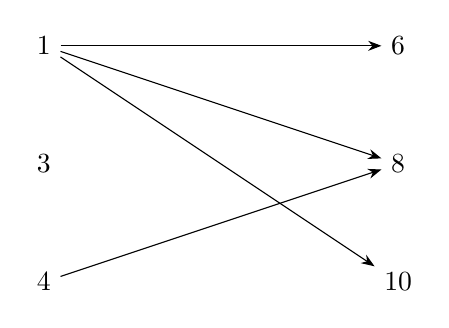
\begin{tikzpicture}[node distance=1.5cm, >=Stealth]
            \node (A1) {1};
            \node (A2) [below of=A1] {3};
            \node (A3) [below of=A2] {4};
            
            \node (B1) [right of=A1, xshift=3cm] {6};
            \node (B2) [below of=B1] {8};
            \node (B3) [below of=B2] {10};
            
            \draw [->] (A1) -- (B1);
            \draw [->] (A1) -- (B2);
            \draw [->] (A1) -- (B3);
            \draw [->] (A3) -- (B2);
        \end{tikzpicture}
    \end{enumerate}
    
    \hrulefill

    \item (10 points) Let $B = \{4, 5, 6\}$ and $A = \{5, 6, 7\}$ and define relations $R$, $S$, and $T$ from $A$ to $B$ as follows:
    \begin{itemize}
        \item For all $(x, y) \in A \times B$, $(x, y) \in R$ means that $x \geq y$.
        \item $(x, y) \in S$ means that $\frac{x - y}{2}$ is an integer.
        \item $T = \{(7, 4), (5, 6), (7, 6)\}$.
    \end{itemize}
    \begin{enumerate}
        \item Draw arrow diagrams for $R$, $S$, and $T$.\\
        \vspace{1em}
        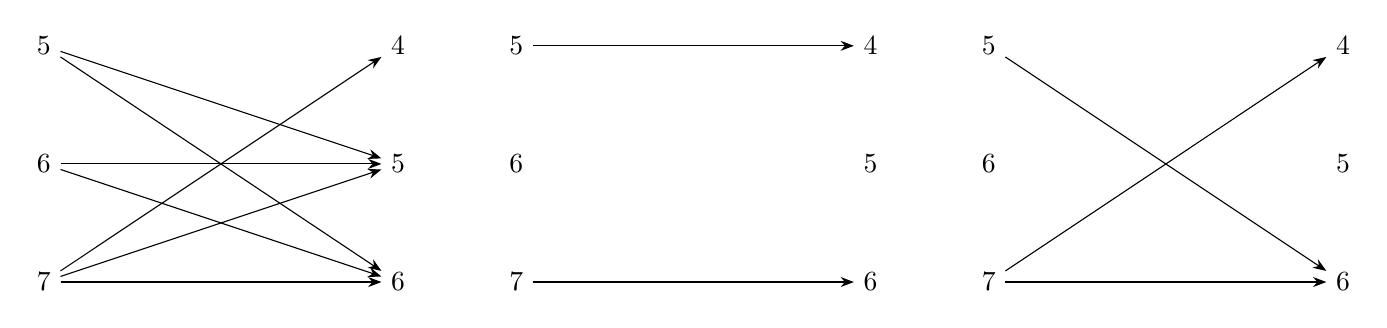
\begin{tikzpicture}[node distance=1.5cm, >=Stealth]
            % Diagram for R
            \node (A1) {5};
            \node (A2) [below of=A1] {6};
            \node (A3) [below of=A2] {7};
            
            \node (B1) [right of=A1, xshift=3cm] {4};
            \node (B2) [below of=B1] {5};
            \node (B3) [below of=B2] {6};
            
            \draw [->] (A1) -- (B2);
            \draw [->] (A1) -- (B3);
            \draw [->] (A2) -- (B3);
            \draw [->] (A2) -- (B2);
            \draw [->] (A3) -- (B1);
            \draw [->] (A3) -- (B2);
            \draw [->] (A3) -- (B3);

            % Diagram for S
            \begin{scope}[xshift=6cm]
                \node (A1) {5};
                \node (A2) [below of=A1] {6};
                \node (A3) [below of=A2] {7};

                \node (B1) [right of=A1, xshift=3cm] {4};
                \node (B2) [below of=B1] {5};
                \node (B3) [below of=B2] {6};

                \draw [->] (A1) -- (B1);
                \draw [->] (A3) -- (B3);
            \end{scope}

            % Diagram for T
            \begin{scope}[xshift=12cm]
                \node (A1) {5};
                \node (A2) [below of=A1] {6};
                \node (A3) [below of=A2] {7};

                \node (B1) [right of=A1, xshift=3cm] {4};
                \node (B2) [below of=B1] {5};
                \node (B3) [below of=B2] {6};

                \draw [->] (A3) -- (B1);
                \draw [->] (A1) -- (B3);
                \draw [->] (A3) -- (B3);
            \end{scope}
        \end{tikzpicture}
        \vspace{1em}
        
        \hrulefill

        \item Indicate whether any of the relations $R$, $S$, and $T$ are functions.\\
        \vspace{1em}
        $R$ is not a function.\\
        $S$ is not a function.\\
        $T$ is a function.
        \vspace{1em}
    \end{enumerate}
    
    \hrulefill

    \item (10 points) Define a relation $T$ from $\mathbb{R}$ to $\mathbb{R}$ as follows: For all real numbers $x$ and $y$,
    $(x, y) \in T$ means that $y^2 - x^2 = 1$.\\
    \vspace{1em}
    Is $T$ a function? Explain.\\
    \vspace{1em}
    No, $T$ is not a function because for a given $x$, there can be two different values of $y$ (one positive and one negative) that satisfy the equation $y^2 - x^2 = 1$.
    \vspace{1em}

\end{enumerate}

\end{document}
